% chktex-file 44
% chktex-file 8
% chktex-file 24
% chktex-file 13
% chktex-file 29
% chktex-file 31

\documentclass[german,report]{i1thesis}

\usepackage{xcolor,colortbl}
\usepackage{amsmath}
\usepackage{biblatex}
\usepackage{pgfplots}
\usepackage{acronym}
% \usepackage{acro}


\def\theauthor{Fabian Berger, B. Sc.}
\def\theadvisor{Prof.\ Dr.-Ing. Michael Tielemann}

% Es ist möglich mehrere Autoren, Betreuer oder Prüfer einzutragen:
%\def\theadvisor{Some guy, M.Sc., \\ & Some other guy, M.Sc}s
% Wenn gendergerechte Sprache gewünscht ist bzw. bei Autor/Prüfer ein Plural 
% gebraucht wird, lässt sich das Keyword so anpassen:
%\def\textadvisor{Betreuende}

\def\theexaminer{Prof.\ Dr.-Ing. Michael Tielemann}
\def\thetitle{Evaluierung eines Chatbots zur Verbesserung der Informationssicherheit an der FAU\@ Lokale Modelle, Plattformvergleich und Integrationsmöglichkeiten}
\def\theplace{Erlangen}
\def\thedate{\today}

% Diese Befehle ändern das jeweilige Keyword auf der Hauptseite
%\def\germanAuthor{Autor}
%\def\germanBetreuer{Betreuer}
%\def\germanPruefer{Prüfer}


\begin{document}

\makethetitle%

\maketoc%

\newpage
\section{Einleitung}%
\label{sec:einleitung}

Die stetig steigende Relevanz von Informationssicherheit erfordert fortlaufende Innovationen, um einen effektiven Wissensaustausch zu fördern.
In diesem Kontext liegt die Motivation für das vorliegende Masterprojekt in der Entwicklung des folgenden Ansatzes: \\
Die Entwicklung eines barrierefreien und anonymen Dialogs zwischen den Mitgliedern der \ac{FAU} mithilfe eines Chatbots.
Das Hauptziel besteht darin, relevante Informationen zur Informationssicherheit bereitzustellen, ohne dabei die Identität der Fragenden preiszugeben.
Damit soll die Informationssicherheit an der \ac{FAU} passiv durch eine selbstständige Nutzung erhöht werden.

In einer Umgebung mit über 500 Lehrstühlen, die eigene Arbeitsweisen und unterschiedliche Kompetenz- und Arbeitsprofile aufweisen, ist es von entscheidender Bedeutung,
dass Interessierte einen einfachen Zugang zu relevanten Informationen erhalten.
Dieser Zugang soll dazu beitragen, Interessierte zu motivieren, sich intensiver mit dem Thema Informationssicherheit auseinanderzusetzen und somit die Sicherheit der gesamten Universität zu erhöhen.

Die Einrichtung eines zugänglichen Dialogs mit einem Chatbot wird dazu beitragen, dass Studierende und Mitarbeiter der \ac{FAU} leichter auf relevante Informationen zugreifen können.
Dieser Ansatz ist nicht nur darauf ausgerichtet, das Bewusstsein für Informationssicherheit zu schärfen, sondern soll auch dazu beizutragen, dass sich die Sicherheitspraktiken innerhalb der gesamten Universität verbessern.
Angesichts der wachsenden Bedrohungen im digitalen Raum ist es von entscheidender Bedeutung, dass die \ac{FAU} als Institution einen proaktiven Ansatz verfolgt, um die Sicherheit ihrer Daten und Systeme zu gewährleisten.

Durch die Anonymität des Dialogs wird zudem ein geschützter Raum geschaffen, der es den Fragenden ermöglicht, ihre Fragen ohne Sorge vor Reaktionen anderer Personen zu stellen.
Dies senkt die Hemmschwelle und mehr Menschen werden dazu ermutigt, sich aktiv mit dem Thema Informationssicherheit auseinanderzusetzen.
Insgesamt trägt das Projekt somit nicht nur zur individuellen Belehrung bei, sondern hat auch das Potenzial, die kollektive Sicherheitskultur an der \ac{FAU} nachhaltig zu stärken.
Auch die Beantwortung von Fragen in Echtzeit ist ein entscheidender Faktor, um die Wirksamkeit des Chatbots sicherzustellen.

\section{Problemstellung}%
\label{sec:problemstellung}
Die vorliegende Problemstellung fokussiert sich auf die Evaluierung eines Chatbots mit dem Ziel, die Informationssicherheit an der \ac{FAU} zu verbessern.
In Anbetracht der äußerst hohen Relevanz von Informationssicherheit wird die Notwendigkeit betont, innovative Ansätze für den Wissensaustausch innerhalb der \ac{FAU} zu entwickeln.
Hochschulen und Universitäten sind ein bevorzugtes Ziel für Cyberangriffe, da unterschiedliche Rechtegruppen mit möglicherweise infizierten beziehungsweise unsicheren Geräten auf die verschiedenen internen Netzwerke zugreifen.

Insbesondere für Personen, die noch nicht mit dem Thema vertraut sind, gestaltet sich die Suche nach den richtigen Informationen als herausfordernd.
Es wird auf die potenziell unzureichende Zugänglichkeit aktueller Informationsquellen zur Informationssicherheit an der \ac{FAU} hingewiesen.
Dieses Defizit soll durch die Implementierung dieses Chatbots verringert werden.

Der vorgeschlagene Projektplan erstreckt sich über 16 Wochen und sieht verschiedene Phasen wie Recherche, Analyse von lokalen, sowie Cloud-Modellen, Plattformauswahl, Integration und Evaluierung der verschiedenen Systeme vor.
Dabei wird eine durchschnittliche Bearbeitungszeit von 20 Stunden pro Woche angesetzt.
Das Hauptaugenmerk liegt darin, das beste System für diese Aufgabe herauszuarbeiten.

\subsection{Thematischer Schwerpunkt}%
\label{subsec:thematischer-schwerpunkt}

Die Themenschwerpunkte des Chatbots umfassen verschiedene Bereiche der Informationssicherheit, die für die \ac{FAU} relevant sind.

Neben konventionellen Chatbots, die nach festen Regeln aufgebaut sind, können auch \acp{LLM} für die Erstellung von Chatbots verwendet werden.
Nach kurzer Prüfung von konventionellen Chatbots, wie beispielsweise Bot Libre \autocite{botlibre}, wurde festgestellt, dass diese nicht die gewünschte Genauigkeit und Anpassungsfähigkeit bieten.
Vor allem der initiale Aufwand für die Erstellung von Regeln und die Wartung des Systems stellte sich als zu hoch heraus, um ein System zu erhalten, welches den Anforderungen wie der dynamischen Anpassbarkeit genügt.

In Rücksprache mit dem Betreuer wurde entschieden, sich auf die Verwendung von \acp{LLM} zu konzentrieren, da diese momentan die fortschrittlichste Technologie im Bereich der Chatbots darstellt.

\section{Zielsetzung}
\label{sec:zielsetzung}

Die konkreten Ziele des Projekts umfassen die Konzeption eines Chatbots, der Fragen zur Informationssicherheit beantwortet.
Vor allem Richtlinien bezüglich geschützter Daten innerhalb der entsprechenden Entität stehen im Fokus der Beantwortung.
Aber auch darüber hinausreichende Themenbereiche können abgedeckt werden, darunter Sicherheitsbewusstsein, Passwortsicherheit, Phishing, Schutz vor Malware und Viren, Identifizierung und Authentifizierung, Datenschutz und -sicherheit \& Netzwerksicherheit.

Diese Lösung soll es ermöglichen, Informationen zur Informationssicherheit und auch dem Datenschutz bereitzustellen, ohne dabei die Identität der Fragenden preiszugeben.
Die Informationen, die der Chatbot zur Beantwortung der Fragen in Betracht ziehen soll, sind in Dokumenten, wie der Informationssicherheitsrichtlinie der \ac{FAU} definiert.

Um diese Informationen leichter zugänglich zu machen, wird evaluiert, welche Plattform hierfür am besten geeignet ist.
Die Auswahl eines geeigneten und leistungsfähigen Modells sowie einer Plattform steht im Fokus des Projektziels.
Die Plattformen werden anhand von Kriterien wie Genauigkeit der Antworten, Benutzerfreundlichkeit, Reaktionszeit, Anpassungsfähigkeit und Sicherheit des Chatbot-Systems bewertet.
Besonderes Augenmerk gilt der Gewährleistung der Anonymität, um die Hemmschwelle für die Nutzer zu minimieren.

\newpage
\section{Vergleich unterschiedlicher Ansätze zur Umsetzung}%
\label{sec:vergleich}

\subsection{Mögliche Betriebsarten des Systems}

Die Implementierung eines solchen Chatbots kann auf unterschiedliche Weise erfolgen.
Eine der größten Unterschiede besteht darin, ob das Modell lokal oder in der Cloud betrieben wird.
Lokale Modelle bieten die Möglichkeit, die Daten und die Verarbeitung lokal zu speichern und zu verarbeiten, während Cloud-Modelle die Verarbeitung und Speicherung online vornehmen.
Die Anonymität der Nutzer zu sichern ist bei lokalen Modellen daher einfacher handhabbar, da die Daten nicht auf externe Server übertragen werden müssen.

Die Performance kann jedoch bei Cloud-Modellen um ein vielfaches höher sein, da die Rechenleistung der Cloud-Anbieter für einen Klienten meist deutlich höher ist als die von lokalen Systemen.
Bei einer Realisierung in der Cloud wäre in jedem Fall ein Thin-Client ausreichend, um den Chatbot zu nutzen.

Da die übertragenen Daten des Systems als schützenswert gesehen werden, muss ein Anbieter gefunden werden, der den Anforderungen zur Datenverarbeitung entsprechen würden.
Das Rechenzentrum der Uni \autocite{rrze} wäre hier sicher ein geeigneter Anbieter, solange das System nicht öffentlich zugänglich ist.
Da die Nutzer hier potenziell sensible Daten preisgeben, ist die Anonymität ein entscheidender Faktor bei der Auswahl des Modells und damit der Gewährleistung der Sicherheit der \ac{FAU}.

Die Wahl des Betriebsmodells hängt daher von verschiedenen Faktoren ab, darunter den Anforderungen an die Sicherheit, die Leistungsfähigkeit der Hardware und die aufkommenden Kosten.




\subsection{Einführung in große Sprachmodelle (LLM)}

\subsubsection{Grundlagen der Sprachmodelle}

\acfp{LLM} sind neuronale Netze, die darauf trainiert sind, Texte auf der Grundlage großer Mengen an Textdaten zu generieren und zu verstehen.
Diese Modelle nutzen maschinelles Lernen, um Muster und Strukturen in den Trainingsdaten zu erkennen und auf neue Texte anzuwenden.
\acp{LLM} bestehen aus tiefen neuronalen Netzen mit Milliarden von Parametern, die während des Trainings angepasst werden, um die Vorhersagegenauigkeit zu maximieren.

Ein entscheidendes Merkmal von \acp{LLM} ist ihre Fähigkeit, kontextuelle Informationen für die Generierung einer Antwort zu nutzen.
Die Entwicklung von \acp{LLM} basiert auf fortschrittlichen Techniken wie der Transformer-Architektur, die die Effizienz und Leistungsfähigkeit von Sprachmodellen erheblich verbessert hat.
\acp{LLM} werden durch Pre-Training auf großen Textdatensätzen und anschließendes Finetuning für spezifische Aufgaben trainiert.

\subsubsection{Architektur der Sprachmodelle}

\acp{LLM} basieren heutzutage meistens auf der sogenannten Transformer-Architektur, die besonders gut für Sprachverarbeitungsaufgaben geeignet ist.
Diese Architektur wurde 2017 durch das Paper \textquote{Attention is All You Need} von Vaswani et al. \autocite{attention} eingeführt und hat seitdem zu einer Revolution in der Sprachverarbeitung geführt.
Nachfolgend ist beispielhaft ein Modell eines Transformers dargestellt:\\

\begin{figure}[H]
    \centering
    \includegraphics[width=0.8\textwidth]{images/The-Transformer-model-architecture.png}
    \caption{Grundsätzliche Transformer Architektur \autocite{yuening2019}}%
    \label{fig:transformer}
\end{figure}


\subsubsection{Anwendungen der Sprachmodelle}


\acp{LLM} finden in einer Vielzahl von Anwendungen Verwendung.\\
Der Anwendungsbereich für diese Modelle wird in Zukunft noch weiter wachsen, wie die vor kurzer Zeit veröffentlichte multimodale Version GPT-4o \autocite{gpt4o} von OpenAI \autocite{openai} zeigt.
Die Anwendungen reichen momentan bereits von der Textgenerierung über die Übersetzung bis hin zur Erstellung von Code, Bildern und kurzen Videos.
Zudem werden sie vermehrt in der Analyse großer Datenmengen und der automatisierten Inhaltsmoderation eingesetzt.
In der Medizin unterstützen \acp{LLM} bei der Diagnosestellung und der personalisierten Patientenversorgung, indem sie medizinische Daten analysieren und relevante Informationen bereitstellen.
Auch im Bildungsbereich finden sie Verwendung, etwa in der Erstellung von personalisierten Lerninhalten.
Diese Vielseitigkeit unterstreicht das Potenzial von \acp{LLM}, in verschiedensten Bereichen signifikante Verbesserungen und Effizienzsteigerungen zu erzielen.

\newpage
\section{Formale Evaluation der Systeme}%
\label{sec:formale-evaluation}

Abgesehen von der Art der Implementierung ist es bei einer Cloud-Lösung wichtig, dass das System für möglichst viele Nutzer gleichzeitig verfügbar ist.
Daher wurde hier für verschiedene Modelle die Anzahl der Parameter, die Anzahl der Wörter und die Zeit, die das Modell für die Beantwortung einer Anfrage benötigt, gemessen.\\


\begin{table}[H]
    \centering
    \begin{tabular}{|l|l|}
        \hline
        \textbf{Parameter} & \textbf{Lokales Setup}                 \\ \hline
        \textbf{\ac{CPU}}  & AMD Ryzen 7 7800X3D                    \\ \hline
        \textbf{\ac{GPU}}  & AMD Radeon 6800XT (16 GB \acs{VRAM})   \\ \hline
        \textbf{\ac{RAM}}  & 32 \acs{GB} DDR5 - 6000 \acs{MHz} CL30 \\ \hline
    \end{tabular}
    \caption{Lokales Testsetup}
\end{table}

Die Ergebnisse sind in der folgenden Tabelle zusammengefasst:\\

\begin{table}[H]
    \centering
    \begin{tabular}{|l|l|l|l|l|}
        \hline
        \textbf{Modell}                                              & \textbf{Parameter (in Mrd.)}            & \textbf{Buchstaben} & \textbf{Zeit (s)} & \textbf{Quotient} \\ \hline
        \textbf{ChatGPT 3.5 (Firefox) \autocite{openai_chatgpt}}     & $\sim$20 \autocite{singh2023codefusion} & 1560                & 11                & 139,7             \\ \hline
        \textbf{Copilot - GPT4 (Edge) \autocite{microsoft_copilot}}  & $\sim$1760 \autocite{decoder2024gpt4}   & 1148                & 35                & 33,5              \\ \hline
        \textbf{Mistral OpenOrca (\ac{GPU}) \autocite{OpenOrca2023}} & 7                                       & 1233                & 11                & 114,7             \\ \hline
        \textbf{Mistral OpenOrca (\ac{CPU}) \autocite{OpenOrca2023}} & 7                                       & 1685                & 110               & 17,7              \\ \hline
        \textbf{Wizard 1.2 (\ac{GPU}) \autocite{WizardLM2023}}       & 13                                      & 1106                & 20                & 54,1              \\ \hline
        \textbf{Wizard 1.2 (\ac{CPU}) \autocite{WizardLM2023}}       & 13                                      & 1072                & 89                & 12                \\ \hline
        \textbf{Hermes (\ac{GPU}) \autocite{NousResearch2023}}       & 13                                      & 7518                & 11                & 61,1              \\ \hline
        \textbf{Hermes (\ac{CPU}) \autocite{NousResearch2023}}       & 13                                      & 805                 & 98                & 8,2               \\ \hline
    \end{tabular}
    \caption{Über 10 Tests gemittelte Werte}
\end{table}

Daraus wird ersichtlich, dass bei einer reinen Verwendung der \ac{CPU} die Modelle um ein Vielfaches langsamer sind als bei einer \ac{GPU}.
Für den Prozess der Textgenerierung, der Inference genannt wird, können im Regelfall \acp{GPU} beider großer Hersteller verwendet werden.
% Auch wird ersichtlich, dass die Performance stark abfällt, sobald das gesamte Modell nicht mehr in den Grafikspeicher passt und damit auf den langsameren Arbeitsspeicher ausweichen muss.
% Der Grafikspeicher ist in jedem Fall entscheidend und sollte so groß wie möglich gewählt werden, um ein möglichst großes Modell verwenden zu können.

\newpage
\section{Anpassung der Systeme auf den Anwendungszweck}%
\label{sec:anpassungen-systeme}

\acp{LLM} lassen sich durch verschiedene Ansätze dem Verwendungszweck anpassen, die teilweise auch in Kombination miteinander verwendet werden können.
Das sogenannte Finetuning ist ein Ansatz, bei dem ein bereits trainiertes Modell mit spezifischen Trainingsdaten angepasst wird.
Dafür sind gut ausgewählte und qualitativ hochwertige Trainingsdaten notwendig, die repräsentativ für den Anwendungsfall sind.
Techniken, die hierbei zum Einsatz kommen, sind vielfältig und entwickeln sich schnell weiter.
Bei dieser Recherche wurden unter anderem \ac{QLoRA}, \ac{PEFT}, Quantisierungen und Mixed-Precision verwendet.\\

Alternativ lässt sich ein Modell auch live durch \ac{RAG} oder Prompt Engineering modifizieren.

\subsection{Finetuning}%
\label{subsec:Finetuning-cloud}

\ac{CUDA} ist eine von Nvidia entwickelte proprietäre Programmierschnittstelle, die es ermöglicht, parallele Berechnungen auf Grafikkarten durchzuführen.
\ac{CUDA} ist an vielen Stellen des Finetunings notwendig, deshalb konnte das Finetuning nicht auf einer mir lokal zur Verfügung stehenden AMD Radeon 6800XT durchgeführt werden.


PyTorch \autocite{pytorch} ist eine Open-Source-Bibliothek für maschinelles Lernen, die von Facebook entwickelt wird.
Sie bietet eine Vielzahl von Funktionen und Werkzeugen, die für das Training von neuronalen Netzwerken verwendet werden können und bietet die Grundlage für die Implementierung von Machine Learning Modellen.

PyTorch bietet zwar mittlerweile auch Unterstützung für  \ac{ROCm}, jedoch sind die Treiber für Teile der Bibliothek den Hochleistungsgrafikkarten vorbehalten und konnte daher von mir nicht getestet werden. \autocite{rocm-support}

Es gibt zwar seit kurzer Zeit auch mit ZLuda \autocite{zluda} eine Möglichkeit, \ac{CUDA} auf AMD-Grafikkarten zu verwenden, jedoch ist diese noch nicht ausgereift und konnte nicht erfolgreich getestet werden.

Finetuning in der Cloud kann bereits durch mehrere Anbieter, wie Kaggle und Google Colab kostenlos durchgeführt werden.
Die Hauptbeschränkung dabei ist der verfügbare Grafikspeicher (\ac{VRAM}), der dabei auf 15 bzw. 16 \ac{GB} beschränkt ist.
Auch die Laufzeit eines Programms ist jeweils begrenzt, was die produktive Nutzung einschränkt.
Hierbei kommen Nvidia Grafikkarten, wie die T4 und die Tesla P100 zum Einsatz.

Diese können gut zu Testzwecken verwendet werden, um Programmcode zu entwickeln und zu testen.
Für den produktiven Einsatz sind jedoch Grafikkarten mit mehr Leistung und mehr Grafikspeicher notwendig.

\newpage
\subsubsection{Finetuning Prozess}%
\label{subsec:Finetuning-prozess}

Um das Modell zu feintunen, wurden verschiedene Ansätze getestet.
Dabei wurde das Modell auf verschiedene Trainingsdaten angepasst und die Ergebnisse ausgewertet.

Der Prozess mit dem besten Erfolg wird im Folgenden genauer beschrieben:

Die entscheidenden Bibliotheken sind dabei PyTorch, sowie Trainer aus dem Transformers-Paket von Huggingface \autocite{huggingface}.

\ac{SFTTrainer} \autocite{sfttrainer} ist ein Trainer aus der Klasse der Huggingface-Trainer für Transformer-Modelle.
\ac{SFT} ist eine Unterart der Trainer-Klasse.

Trainer und \ac{SFTTrainer} sind Huggingface-Klassen, die zum Trainieren von Transformers-Modellen verwendet werden, jedoch unterschiedliche Zwecke erfüllen.
Die Trainer-Klasse ist für allgemeines Training konzipiert und eignet sich vor allem zum Trainieren von Modellen von Grund auf.
Sie bietet eine hohe Anpassbarkeit mit einer breiten Palette an Konfigurationsoptionen zur Feinabstimmung von Hyperparametern, Optimierern, Schedulern, Logging und Evaluationsmetriken.
Zudem unterstützt sie komplexe Trainingsabläufe wie Gradientenakkumulation, Checkpointing und verteiltes Training.
Allerdings erfordert der Trainer in der Regel größere Datensätze für ein effektives Training.

Im Gegensatz dazu ist der \ac{SFTTrainer} für das überwachtes Finetuning (\ac{SFT}) optimiert und eignet sich besonders für das Finetuning vortrainierter Modelle mit kleineren Datensätzen.
Er bietet eine einfachere Schnittstelle mit einem vereinfachten Workflow und weniger Konfigurationsoptionen, was den Einstieg erleichtert.
Der \ac{SFTTrainer} nutzt ebenso effiziente Speichertechniken wie \ac{PEFT} und Optimierungen zur Reduzierung des Speicherverbrauchs während des Trainings.

Zusammenfassend bietet der \ac{SFTTrainer} eine einfachere und effizientere Möglichkeit, vortrainierte Modelle mit kleinen Datensätzen zu feintunen, während die Trainer-Klasse eine größere Flexibilität und Anpassbarkeit für das Training bietet.
Daher wird im Folgenden nur noch der \ac{SFTTrainer} betrachtet.

\subsubsection{Erklärung der verwendeten Techniken}%

\ac{PEFT} beschreibt eine Methode zur Reduzierung des Speicherverbrauchs während des Trainings mittels \ac{QLoRA}.
\ac{QLoRA} basiert auf \ac{LoRA} und sind Techniken, die die Größe des Modells durch Quantisierung reduzieren, um den Speicherverbrauch weiter zu verringern.
\ac{LoRA} modifiziert den Finetuning-Prozess, indem es die ursprünglichen Modellgewichte einfriert und Änderungen an einem separaten, zusätzlichen Satz von Gewichten vornimmt, die dann zu den ursprünglichen Parametern hinzugefügt werden.

\begin{figure}[H]
    \centering
    \includegraphics[width=0.95\textwidth]{images/qlora.jpg}
    \caption{Vergleich der verschiedenen Techniken \autocite[S. 3]{qlora}}%
    \label{fig:qlora}
\end{figure}

Des Weiteren wird Mixed-Precision Computing verwendet, um die Berechnungen zu beschleunigen und den Speicherverbrauch zu reduzieren.

Im Finetuning-Prozess können verschiedene Genauigkeitsformate verwendet werden.
Die gängigsten Formate sind das \ac{FP16}, das \ac{FP32} und das \ac{FP64}.
Seit der Ampere-Generation von Nvidia Grafikkarten wird auch das \ac{BF16} unterstützt, welches eine Mischung aus \ac{FP16} und \ac{FP32} darstellt.

\ac{BF16} hat die gleiche Anzahl an Exponentenbits wie \ac{FP32}, jedoch die Gesamtbitanzahl von \ac{FP16}.
Dies führt zu einem geringeren Speicherbedarf und gleichzeitig schnellerem Training bei gleichzeitig vergleichbarer Genauigkeit wie \ac{FP32}.
\textquote{We can see that using \ac{BF16} increases training throughput by 18 \% and is significantly less prone to weight growth.} \autocite{bf16}

Ein Vergleich der Techniken ist in der folgenden Tabelle dargestellt:

\begin{figure}[H]
    \centering
    \includegraphics[width=1\textwidth]{images/bf16.png}
    \caption{Vergleich der verschiedenen Genauigkeitsformate \autocite{bf16-pic}}%
    \label{fig:bf16}
\end{figure}


Für den Finetuning Prozess benötigt man zunächst ein vortrainiertes Modell, sowie einen Datensatz, der für das Finetuning verwendet werden soll.

Hier wurde zu Testzwecken beispielhaft das Llama-2-7b-chat-hf Modell von NousResearch \autocite{NousResearch2023-2} und der Datensatz Guanaco-llama2-1k von Mlabonne \autocite{mlabonne2023} verwendet.
Die Chat-Variante des Modells wurde gewählt, da diese speziell für die Beantwortung von Fragen optimiert ist.
Andere Modelle verwenden hier analoge Begriffe, wie \textquote{it} oder \textquote{instruct} für \textquote{Instruktion}.


\subsubsection{Erklärung des Training-Prozesses}%
\label{subsec:training-prozess}

Zuerst werden die notwendigen Bibliotheken installiert.\\

\begin{table}[H]
    \centering
    \begin{tabular}{|l|l|}
        \toprule
        \textbf{Paket} & \textbf{Version} \\ \midrule
        accelerate     & 0.21.0           \\
        peft           & 0.4.0            \\
        bitsandbytes   & 0.40.2           \\
        transformers   & 4.31.0           \\
        trl            & 0.4.7            \\ \bottomrule
    \end{tabular}
    \caption{Installation der erforderlichen Pakete}
    \label{tab:installation}
\end{table}

Daraufhin wird das Modell, der Datensatz und der Tokenizer geladen.

Das Modell wird dabei mit reduzierter 4-Bit-Präzision geladen, um die Speicheranforderungen zu minimieren, wie bereits im Finetuning-Prozess in~\ref{subsec:Finetuning-prozess} beschrieben.\\

\begin{lstlisting}[language=Python]
    bnb_config = BitsAndBytesConfig(
        load_in_4bit=use_4bit,
        bnb_4bit_quant_type=bnb_4bit_quant_type,
        bnb_4bit_compute_dtype=torch.float16,
        bnb_4bit_use_double_quant=use_nested_quant,
    )
\end{lstlisting}

Anschließend wird die Konfiguration für das \ac{QLoRA}-Verfahren geladen.\\

\begin{lstlisting}[language=Python]
    peft_config = LoraConfig(
        lora_alpha=lora_alpha,
        lora_dropout=lora_dropout,
        r=lora_r,
        bias="none",
        task_type="CAUSAL_LM",
    )
\end{lstlisting}

Als Nächstes werden die Trainingsparameter definiert, einschließlich der Anzahl der Epochen, der Batchgröße und der Lernrate.
Diese Parameter sind entscheidend für die Feinabstimmung und die Optimierung des Modells und beeinflussen den Erfolg des Trainingsprozesses maßgeblich.\\

\begin{lstlisting}[language=Python]
training_arguments = TrainingArguments(
    output_dir=output_dir,
    num_train_epochs=num_train_epochs,
    per_device_train_batch_size=per_device_train_batch_size,
    gradient_accumulation_steps=gradient_accumulation_steps,
    optim=optim,
    save_steps=save_steps,
    logging_steps=logging_steps,
    learning_rate=learning_rate,
    weight_decay=weight_decay,
    fp16=fp16,
    bf16=bf16,
    max_grad_norm=max_grad_norm,
    max_steps=max_steps,
    warmup_ratio=warmup_ratio,
    group_by_length=group_by_length,
    lr_scheduler_type=lr_scheduler_type,
    report_to="tensorboard"
)
\end{lstlisting}

Der \ac{SFT}Trainer wird mit allen geladenen Konfigurationen und Parametern initialisiert. Diese Trainer-Instanz übernimmt den eigentlichen Finetuning-Prozess.
Diesem werden alle bereits vorher definierten Parameter übergeben.\\

\begin{lstlisting}[language=Python]

trainer = SFTTrainer(
model=model,
train_dataset=dataset,
peft_config=peft_config,
dataset_text_field="text",
max_seq_length=max_seq_length,
tokenizer=tokenizer,
args=training_arguments,
packing=packing,
)
trainer.train()

\end{lstlisting}

Nach dem Training wird das fertige Modell gespeichert, sodass es für zukünftige Inferenz und Weiterentwicklungen verwendet werden kann.

Auch die lokale Inferenz wird mithilfe von Huggingface realisiert.

Zuerst wird das Modell und der Tokenizer in den Grafikspeicher geladen.\\

\begin{lstlisting}[language=Python]
model = AutoModelForCausalLM.from_pretrained(model_name, load_in_4bit=True)
model = PeftModel.from_pretrained(model, adapter_model_name)
tokenizer = AutoTokenizer.from_pretrained(model_name, use_fast=True)
\end{lstlisting}

Die Trainingsdaten werden aus einer \ac{JSONL}-Datei (\texttt{ts\_train.jsonl}) geladen.
Jede Zeile der Datei enthält einen Text, der in den Teil der Frage (\texttt{human\_text}) und den Teil der erwarteten Antwort (\texttt{assistant\_text}) aufgeteilt wird.
Die ersten 10 Wörter der erwarteten Antwort werden im \texttt{assistant\_array} gespeichert.\\

\begin{lstlisting}[language=Python]
with open("./ts_train.jsonl", "r") as file:
for line in file:
    json_data = json.loads(line)
    human_text = json_data["text"].split("### Assistant: ")[0].split("### Human: ")[1]
    human_array.append(human_text)
    assistant_text = json_data["text"].split("### Assistant: ")[1]
    first_10_words = ' '.join(assistant_text.split()[:10])
    assistant_array.append(first_10_words)
\end{lstlisting}



Die Inferenz wird in einer Schleife durchgeführt, die die Anzahl der Durchläufe bestimmt, wobei jede Frage einzeln verarbeitet wird und die Zeit für die Verarbeitung gemessen wird.
Ein Tokenizer wird verwendet, um die Eingaben zu verarbeiten und auf eine \ac{CUDA}-\ac{GPU} zu übertragen.
Nach der Generierung der Antwort wird diese dekodiert und mit der erwarteten Antwort verglichen.\\


\begin{lstlisting}[language=Python]for i in range(passes):
for i, question in enumerate(human_array):
    start_time = time.time()

    inputs = tokenizer(question, return_tensors="pt").to("cuda:0")
    output = model.generate(**inputs, min_length=50, max_length=300)

    end_time = time.time()
    times.append(end_time - start_time)
    print(f"Time taken for question {i+1}: {end_time - start_time} seconds")
    print("CHECKING ANSWER: ")
    print("Expected: " + assistant_array[currentQuestion])
    print("Actual: " + tokenizer.decode(output[0], skip_special_tokens=True))
    if assistant_array[currentQuestion] in tokenizer.decode(output[0], skip_special_tokens=True):
        points += 1
        print("CORRECT ANSWER! (" + str(points) + " / " + str(currentQuestion+1) + ")")
    currentQuestion += 1
\end{lstlisting}


% Hier erstmal das Llama-2-7b-hf mit mlabonne/guanaco-llama2-1k
% Geht über colab, nur zeitliche begrenzung, muss also schnell sein

% -LLMs:
% -Optimierung durch Finetuning eines Modells mit spezifischen Trainingsdaten
% -Optimierung durch Anpassung der Hyperparameter
% -Optimierung durch Anpassung der Architektur
% -Optimierung durch Anpassung der Trainingsdauer
% -Parameter: Datenauswahl, Datenvorbereitung, Datenformat, Trainingsparameter, Trainingsbibliothek

% .AI Paper Is a Gem For Model Trainers
% \url{https://www.reddit.com/r/LocalLLaMA/comments/1b9kq9v/01ai_paper_is_a_gem_for_model_trainers/?share_id=yOKtViA_zhHHH0sJ7OIwX&utm_content=1&utm_medium=android_app&utm_name=androidcss&utm_source=share&utm_term=3}

% Reddit: \url{https://www.reddit.com/r/LocalLLaMA/comments/14vnfh2/my_experience_on_starting_with_fine_tuning_llms/}
% How to finetune with Huggingface: \url{https://www.philschmid.de/fine-tune-llms-in-2024-with-trl#5-test-and-evaluate-the-llm}
% Hawki: \url{https://ai.hawk.de/login.php}
% ddp Ressources: \url{https://nvidia-merlin.github.io/Transformers4Rec/stable/multi_gpu_train.html}


Um mehrere \acp{GPU} zu verwenden, wird \ac{DP}, sowie \ac{DDP} verwendet.\\
\ac{DP} ist ein Single-Process, Multi-Thread Ansatz und funktioniert nur auf einer einzigen Maschine.
\ac{DDP} hingegen ist ein Multi-Process Ansatz, der sowohl auf Einzel- als auch auf Multi-Maschinen-Training ausgelegt ist.
\ac{DDP} ist in der Regel schneller als \ac{DP}, da es \ac{GIL}-Engpässe und zusätzlichen Overhead vermeidet.
Bei sehr großen Modellen, die nicht auf eine einzelne \ac{GPU} passen, kann \ac{DDP} mit Model Parallel kombiniert werden, was bei \ac{DP} nicht möglich ist. \autocite{ddp}


Im Colab Notebook hat der Code dafür erfolgreich funktioniert.
Mit Ressourcen des Rechenzentrums wurden diese Techniken erst im \ac{HPC}-Cluster (Jupyter) getestet, was aber noch nicht zum gewünschten Erfolg geführt hat.
Der Lösung des Problems lag daran, wie die \acp{GPU} angesprochen wurden und kann in dieser Quelle weiter verfolgt werden. \autocite{problem}

% Daher DDP einbauen, unterschied zu dp erklären (\url{https://huggingface.co/docs/trl/sft_trainer#multi-gpu-training}) (\url{https://pytorch.org/tutorials/intermediate/ddp_tutorial.html})

% Bisschen Probleme das auf einem Rechencluster mit jeweils 11GB VRAM zum laufen zu bringen -> (\url{https://github.com/huggingface/accelerate/issues/1840#issuecomment-1683105994}) (normal ausführen mit python, mit deviceUNDERSCOREmap='auto' --> Also Naive PP) --> funktioniert erstmals, aber nutzt wohl nur CUDA von einer GPU? -> also scheisse???
% DA in dem Link steht auch dabei wie ich das zum laufen bekomme ohne NPP (also dann schneller mit x*CUDA) wenn ich auf einem besseren Cluster arbeite.

Eine Auflistung weiterer Optimierungen, die in der Zukunft getestet werden können, ist in der folgenden Tabelle dargestellt:
% noch weitere Optimierungen (\url{https://huggingface.co/docs/transformers/perf_train_gpu_one#mixed-precision-training})

\begin{table}[H]
    \centering
    \begin{tabular}{>{\raggedright\arraybackslash}m{6cm} >{\centering\arraybackslash}m{4cm} >{\centering\arraybackslash}m{4cm}}
        \toprule
        \textbf{Methode/Werkzeug}         & \textbf{Verbessert Trainingsgeschwindigkeit} & \textbf{Optimiert Speichernutzung} \\
        \midrule
        Wahl der Batchgröße               & Ja                                           & Ja                                 \\
        Gradientenakkumulation            & Nein                                         & Ja                                 \\
        Gradienten-Checkpointing          & Nein                                         & Ja                                 \\
        Training mit gemischter Präzision & Ja                                           & (Nein)                             \\
        Wahl des Optimierers              & Ja                                           & Ja                                 \\
        Datenvorabladung                  & Ja                                           & Nein                               \\
        DeepSpeed Zero                    & Nein                                         & Ja                                 \\
        torch.compile                     & Ja                                           & Nein                               \\
        \ac{PEFT}                         & Nein                                         & Ja                                 \\
        \bottomrule
    \end{tabular}
    \caption{Vergleich von Methoden/Werkzeugen zur Verbesserung der Trainingsgeschwindigkeit und Optimierung der Speichernutzung, Quelle: \autocite{tabelle-hf}}
    \label{table:vergleich}
\end{table}



\subsubsection{Durchführung der Tests}%
\label{subsec:durchfuehrung-der-tests}

Bevor mit dem Training begonnen werden kann, muss vorher ein Datensatz für das Training erstellt werden.
Hierfür wurde ein testweise ein \ac{JSONL}-Datensatz mit Texten aus Musikstücken genommen.
Diese sind aufgrund von Urheberrechten nicht im ursprünglichen Modell enthalten.
Damit kann ausgeschlossen werden, dass das Modell diese Daten bereits kennt und somit die Ergebnisse nicht durch das Wiederholen von Trainingsdaten beeinflusst werden.
Nach dem Einfügen der Daten in den Datensatz wird dieser in das benötigte Format umgewandelt und anschließend wahlweise auf Huggingface hochgeladen oder lokal gespeichert.

Der Algorithmus für dieses Vorgehen ist im Folgenden dargestellt:

\begin{lstlisting}[language=Python]
from datasets import load_dataset
import re

dataset = load_dataset('user/dataset_name')
dataset = dataset['train'].shuffle(seed=42)

def transform_conversation(example):
    conversation_text = example['text']
    segments = conversation_text.split('###')
    reformatted_segments = []

    for i in range(1, len(segments) - 1, 2):
        human_text = segments[i].strip().replace('Human:', '').strip()

        if i + 1 < len(segments):
            assistant_text = segments[i+1].strip().replace('Assistant:', '').strip()
            reformatted_segments.append(f'<s>[INST] {human_text} [/INST] {assistant_text} </s>')
        else:
            reformatted_segments.append(f'<s>[INST] {human_text} [/INST] </s>')

    return {'text': ''.join(reformatted_segments)}

transformed_dataset = dataset.map(transform_conversation)
\end{lstlisting}

Nachdem der Datensatz erstellt wurde, kann das Training durchgeführt werden.

\subsubsection{Analyse der gegebenen Antworten}%
\label{subsec:Analyse der gegebenen Antworten}
% ----------------sft2.py

% 5 Tests mit 2080ti und 2 GPUs:
% Durchschnitt von 725,721, 721, 742,746 = 731
% Varianz = 116,4
% Standardabweichung = 10,8

% Da kleine Standardabweichung -> ab jetzt nur noch 1 Test pro Szenario.

Bei dem ersten Test wird die Parallelisierung mithilfe von \ac{NPP} umgesetzt.
\ac{NPP} ist die Standardeinstellung und der einfachste Ansatz, um ein Modell auf mehrere \acp{GPU} zu verteilen.

\begin{figure}[H]
    \centering
    \includegraphics[width=0.8\textwidth]{images/npp.png}
    \caption{Funktionsweise von \acl{NPP}}%
    \label{fig:npp}
\end{figure}

Das Ergebnis beschreibt dabei die benötigte Zeit in Sekunden für die Durchführung des Trainings.
% NPP ohne Bfloat16 ohne FP16 (ab Pascal, also alle (TODO?))     FP16 = mixed precision!         BF16 support = Ampere GPU mit cuda>=11.0
\begin{table}[H]
    \centering
    \renewcommand{\arraystretch}{1.5}
    \begin{tabular}{|c|c|c|c|c|c|}
        \hline
                    & 2080TI                & 3080                     & V100                     & A100                    \\
        \hline
        1 \ac{GPU}  & \cellcolor{gray}NaN   & \cellcolor{gray}NaN      & \cellcolor{yellow!50}523 & \cellcolor{green!50}255 \\
        \hline
        2 \acp{GPU} & \cellcolor{red!50}731 & \cellcolor{yellow!50}575 & \cellcolor{yellow!50}530 & \cellcolor{green!50}257 \\
        \hline
        3 \acp{GPU} & \cellcolor{red!50}727 & \cellcolor{yellow!50}581 & \cellcolor{yellow!50}538 & \cellcolor{green!50}260 \\
        \hline
        4 \acp{GPU} & \cellcolor{red!50}734 & \cellcolor{yellow!50}584 & \cellcolor{yellow!50}543 & \cellcolor{green!50}262 \\
        \hline
    \end{tabular}
    \caption{Ergebnisse des Trainings}
\end{table}

Mithilfe von \ac{FP16} und \ac{BF16} konnte die Performance weiter gesteigert werden.
Dabei ist zu beachten, dass \ac{BF16} ab der Ampere-Generation mit \ac{CUDA}-Versionen ab 11.0 unterstützt wird.

\begin{table}[H]
    \centering
    \renewcommand{\arraystretch}{1.5}
    \begin{tabular}{|c|c|c|c|c|c|c|c|}
        \hline
                    & 2080TI-\ac{FP16}      & 3080-\ac{FP16}           & 3080-\ac{BF16}           & V100-\ac{FP16}           & A100-\ac{FP16}          & A100-\ac{BF16}          \\
        \hline
        1 \ac{GPU}  & \cellcolor{gray}NaN   & \cellcolor{gray}NaN      & \cellcolor{gray}NaN      & \cellcolor{yellow!50}481 & \cellcolor{green!50}221 & \cellcolor{green!50}220 \\
        \hline
        2 \acp{GPU} & \cellcolor{red!50}669 & \cellcolor{yellow!50}555 & \cellcolor{yellow!50}599 & \cellcolor{yellow!50}501 & \cellcolor{green!50}244 & \cellcolor{green!50}242 \\
        \hline
        4 \acp{GPU} & \cellcolor{red!50}690 & \cellcolor{yellow!50}556 & \cellcolor{yellow!50}603 & \cellcolor{yellow!50}520 & \cellcolor{green!50}261 & \cellcolor{green!50}259 \\
        \hline
    \end{tabular}
    \caption{Ergebnisse des Trainings}
\end{table}
Die Consumer-\acp{GPU} wurden nicht mehr einzeln getestet, weil die Ergebnisse aufgrund von \ac{NPP} identisch sind.


% Für die Inference wurden die folgenden Ergebnisse erzielt:

% \begin{table}[H]
%     \centering
%     \renewcommand{\arraystretch}{1.5}
%     \begin{tabular}{|c|c|c|c|c|c|}
%         \hline
%                & 2080ti                  & 2080ti mit accelerate    & V100                 & A100                 \\
%         \hline
%         1 GPU  & \cellcolor{green!50}193 & \cellcolor{gray!50}-/-   & \cellcolor{black!50} & \cellcolor{black!50} \\
%         \hline
%         2 GPUs & \cellcolor{green!50}219 & \cellcolor{yellow!50}320 & \cellcolor{black!50} & \cellcolor{black!50} \\
%         \hline
%         4 GPUs & \cellcolor{green!50}189 & \cellcolor{yellow!50}315 & \cellcolor{black!50} & \cellcolor{black!50} \\
%         \hline
%     \end{tabular}
%     \caption{Ergebnisse der Inference}
% \end{table}


In der folgenden Tabelle sind die subjektiven Ergebnisse der Inferenz-Tests dargestellt:
Ein \textquote{+} steht dabei für ein grundsätzlich gutes Ergebnis, ein \textquote{0} für mittelmäßiges und ein \textquote{-} für ein schlechtes Ergebnis.\\

\begin{table}[H]
    \centering
    \begin{tabular}{|l|c|c|c|c|c|l|}
        \hline
        \textbf{Test} & \textbf{Durchlauf 1} & \textbf{D. 2} & \textbf{D. 3} & \textbf{D. 4} & \textbf{D. 5} & \textbf{Änderungen am Testsetup} \\
        \hline
        1             & -                    & -             & -             & -             & -             & mit Evaluation Datensatz         \\
        \hline
        2             & +                    & +             & +             & +             & +             & ohne Gradient Checkpointing      \\
        \hline
        3             & 0                    & 0             & 0             & 0             & 0             & größeres Modell ausprobiert      \\
        \hline
        4             & +                    & +             & 0             & 0             & +             & 100 statt 10 Epochen             \\
        \hline
        5             & X                    & X             & X             & X             & X             & Fehler (\ac{VRAM}-Limit)         \\
        \hline
    \end{tabular}
    \caption{Ergebnisse der Tests}

\end{table}

Der letzte Test schlug dabei fehl, da die Grafikkarte nicht genügend Speicher für ein Modell mit 70 Billionen Parametern hatte.
Dies war selbst bei einer Nvidia A100 mit 40 \ac{GB} \ac{VRAM} der Fall.
Um die Konsistenz zu überprüfen, wurden die Tests 1, 2 und 4 nochmal wiederholt:


\begin{table}[H]
    \centering
    \begin{tabular}{|l|c|c|c|c|c|}
        \hline
        \textbf{Test} & \textbf{Durchlauf 1} & \textbf{D. 2} & \textbf{D. 3} & \textbf{D. 4} & \textbf{D. 5} \\
        \hline
        1-2           & 0                    & 0             & 0             & -             & -             \\
        \hline
        2-2           & 0                    & 0             & 0             & 0             & 0             \\
        \hline
        4-2           & +                    & 0             & +             & 0             & +             \\
        \hline
    \end{tabular}
    \caption{Ergebnisse der Konsistenz-Tests}
\end{table}


% Dann zur Kontrolle nochmal mit 3*760: +|+|+
% Dann zur Kontrolle nochmal mit 3*880: 0|0|0

Unter anderem wurde die Anzahl der Epochen variiert, um zu sehen, wie sich die Trainingsdauer und die Ergebnisse verändern.
Die notwendige Anzahl an Epochen lässt sich gut durch die Loss-Funktion bestimmen.
Dieser nach zu urteilen sind 5 Epochen ausreichend, um ein optimales Ergebnis zu erzielen.

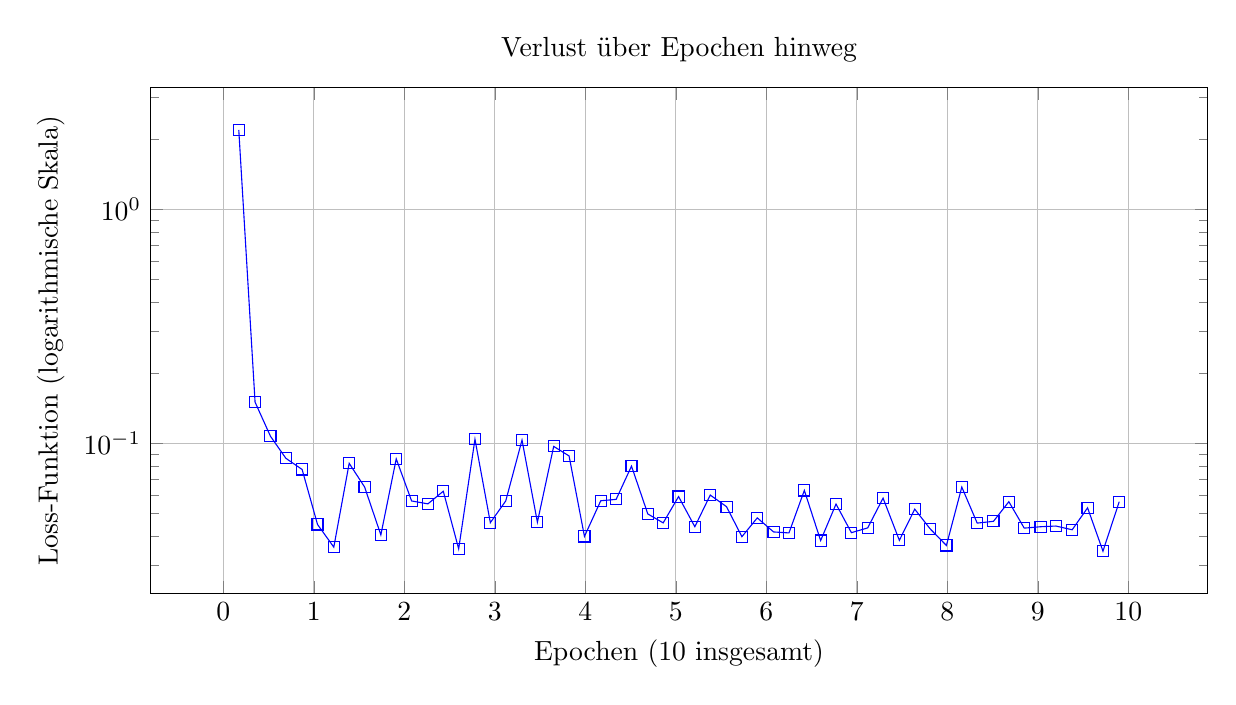
\begin{tikzpicture}
    \begin{axis}[
            title={Verlust über Epochen hinweg},
            xlabel={Epochen (10 insgesamt)},
            ylabel={Loss-Funktion (logarithmische Skala)},
            ymode=log,
            grid=major,
            width=15cm,
            height=8cm,
        ]
        \addplot[
            color=blue,
            mark=square,
        ]
        coordinates {
                (0.17, 2.1822)
                (0.35, 0.1499)
                (0.52, 0.1072)
                (0.69, 0.0863)
                (0.87, 0.0773)
                (1.04, 0.045)
                (1.22, 0.036)
                (1.39, 0.0821)
                (1.56, 0.0651)
                (1.74, 0.0406)
                (1.91, 0.0858)
                (2.08, 0.0567)
                (2.26, 0.0551)
                (2.43, 0.0624)
                (2.6, 0.0354)
                (2.78, 0.1041)
                (2.95, 0.0458)
                (3.12, 0.0567)
                (3.3, 0.1032)
                (3.47, 0.046)
                (3.65, 0.097)
                (3.82, 0.0883)
                (3.99, 0.04)
                (4.17, 0.0568)
                (4.34, 0.0576)
                (4.51, 0.0799)
                (4.69, 0.0499)
                (4.86, 0.0457)
                (5.03, 0.0592)
                (5.21, 0.044)
                (5.38, 0.0601)
                (5.56, 0.0536)
                (5.73, 0.0399)
                (5.9, 0.048)
                (6.08, 0.0418)
                (6.25, 0.0414)
                (6.42, 0.0629)
                (6.6, 0.0384)
                (6.77, 0.055)
                (6.94, 0.0415)
                (7.12, 0.0435)
                (7.29, 0.0583)
                (7.47, 0.0385)
                (7.64, 0.0523)
                (7.81, 0.0431)
                (7.99, 0.0366)
                (8.16, 0.065)
                (8.33, 0.0456)
                (8.51, 0.0464)
                (8.68, 0.0563)
                (8.85, 0.0434)
                (9.03, 0.044)
                (9.2, 0.0443)
                (9.38, 0.0427)
                (9.55, 0.053)
                (9.72, 0.0346)
                (9.9, 0.0563)
            };
    \end{axis}
\end{tikzpicture}

% NEUER TEST:
% 6:111 7b-hf mit 5epochs
% 7:112 7b-chat-hf mit 5epochs
% 8:113 13b-chat-hf mit 5epochs
% 9:114
% 10:


Die subjektive Bewertung der Ergebnisse fällt dabei noch nicht zufriedenstellend aus, weil die Ergebnisse nicht zuverlässig genug waren.
Die Antworten waren oft nicht korrekt oder nicht vollständig.
Auch hat derselbe Trainingszyklus zu unterschiedlichen Ergebnissen geführt.

Abschließend lässt sich zusammenfassen, dass für einen Einsatz des Systems in einer Produktionsumgebung noch deutlich mehr Tests und auch Optimierungen notwendig sind, bevor dieses System produktiv eingesetzt werden kann.

\newpage
\subsection{Retrieval Augmented Generation (RAG)}%
\label{subsec:rag}


\ac{RAG} wurde mit zwei verschiedenen Implementierungen getestet.
GPT4All \autocite{gpt4all} und LM Studio \autocite{lmstudio}, welches über ein Skript angesteuert wird.

GPT4All hat hier allerdings keine brauchbaren Ergebnisse geliefert und wurde daher nicht weiter betrachtet.
Die Implementierung von \ac{RAG} ist nicht gut genug und vor allen Dingen nicht anpassbar genug, um für die Anforderungen dieser Arbeit geeignet zu sein.

LM Studio bietet die Möglichkeit, Modelle direkt von Huggingface zu laden und mithilfe einer einfachen \ac{API} zu verwenden.
Testweise wurde der Webserver nur lokal getestet, aber auch eine Nutzung von außerhalb ist möglich.

Nachfolgend sind die Testparameter des Systems aufbereitet, wie sie in LM Studio verwendet wurden:


\begin{table}[H]
    \centering
    \begin{tabular}{|l|l|}
        \hline
        \textbf{Software}        & \textbf{Version} \\ \hline
        LM Studio (RocM-Version) & 0.2.22           \\ \hline
        RocM Version             & 5.6              \\ \hline
        Windows Version          & 10 - Build 19045 \\ \hline
    \end{tabular}
    \caption{Verwendete Softwareversionen zur Rekonstruktion der Tests}
    \label{tab:software_versions}
\end{table}

Die folgenden Modelle wurden für die Tests verwendet:

\begin{table}[H]
    \centering
    \begin{tabular}{|c|c|c|c|}
        \hline
        \textbf{Param.} & \textbf{Familie} & \textbf{Modell (GGUF-Version)}               & \textbf{Größe (Quant.)}  \\ \hline
        3B              & Phi              & TheBloke/phi-2                               & 1.62 \ac{GB} (Q4\_K\_S)  \\ \hline
        72B             & Llama            & mradermacher/Rhea-72b-v0.5-i1                & 31.04 \ac{GB} (Q2\_K)    \\ \hline
        7B              & Llama            & NousResearch/Hermes-2-Pro-Mistral-7B         & 4.11 \ac{GB} (Q4\_0)     \\ \hline
        2B              & Gemma            & lmstudio-ai/gemma-2b-it                      & 2.67 \ac{GB} (Q8\_0)     \\ \hline
        70B             & Llama            & lmstudio-community/Meta-Llama-3-70B-Instruct & 21.14 \ac{GB} (IQ2\_XS)  \\ \hline
        8B              & Llama            & lmstudio-community/Meta-Llama-3-8B-Instruct  & 4.92 \ac{GB} (Q4\_K\_M)  \\ \hline
        13B             & Llama            & TheBloke/Llama-2-13B-chat                    & 10.68 \ac{GB} (Q6\_K)    \\ \hline
        34B             & Llama            & TheBloke/OrionStar-Yi-34B-Chat-Llama         & 14.96 \ac{GB} (Q3\_K\_S) \\ \hline
        7B              & Llama            & TheBloke/Mistral-7B-Instruct-v0.2            & 4.14 \ac{GB} (Q4\_K\_S)  \\ \hline
    \end{tabular}
    \caption{Verwendete Modelle für die nachfolgenden Tests}%
    \label{tab:verwendete_modelle}
\end{table}

Für die Verwendung der Llama 3 Modelle wird das Nutzen des Llama 3 Vorlagen empfohlen, da die Modelle sonst nicht korrekt geladen werden \autocite{llama3_preset}.
In Kombination mit dem Setup für Retrieval Augment Generation (\ac{RAG}) haben diese Modelle allerdings nicht korrekt gearbeitet.
Nach der Erstellung eines eigenen Templates für diese Modellfamilie konnten die Modelle korrekt geladen und verwendet werden.



\subsubsection{RAG-Algorithmus}%
\label{subsec:rag-alg}

\begin{lstlisting}[language=Python]
    client = OpenAI(base_url="http://localhost:1234/v1", api_key="lm-studio")
    \end{lstlisting}
Hier wird ein OpenAI-Client initialisiert, der zur Kommunikation mit einem lokal laufenden Sprachmodell verwendet wird.


\begin{lstlisting}[language=Python]
    mydir = Path.home() / 'rag' / 'data' / 'info' / 'FAU Richtlinie zur Informationssicherheit v0.95.txt'
    loader = TextLoader(mydir.absolute(), encoding='utf-8')
    data = loader.load()
    \end{lstlisting}
Der Pfad zu der zu verwendenden Quelldatei wird definiert und die Datei wird geladen.


\begin{lstlisting}[language=Python]
    text_splitter = RecursiveCharacterTextSplitter(chunk_size=1000, chunk_overlap=200)
    splits = text_splitter.split_documents(data)
    embedding = FastEmbedEmbeddings()
    vectorstore = Chroma.from_documents(documents=splits, embedding=embedding)
    retriever = vectorstore.as_retriever()
    \end{lstlisting}
Der geladene Text wird in kleinere Abschnitte aufgeteilt, um effizient verarbeitet zu werden. Dann werden Einbettungen für diese Abschnitte erstellt und in einem Vektorspeicher abgelegt.


\begin{lstlisting}[language=Python]
    template = """Beantworten Sie die Frage am Ende des Textes anhand der bereitgestellten Informationen.
    Wenn Sie die Antwort nicht wissen, sagen Sie einfach, dass Sie es nicht wissen, versuchen Sie nicht, eine Antwort zu erfinden.
    Fassen Sie sich bei der Antwort so kurz wie möglich.
    
    KONTEXT:
    
    ```{context}```
    
    FRAGE: {question}
    
    ANTWORT:"""
    custom_rag_prompt = PromptTemplate.from_template(template)
    prompt = ChatPromptTemplate.from_template(template)
    \end{lstlisting}
Eine Vorlage für die Fragestellung wird definiert, die den Kontext und die Frage enthält.

\begin{lstlisting}[language=Python]
    def enter_question(question_text=None):
        rag_chain = (
            {"context": retriever | format_docs, "question": RunnablePassthrough()}
            | prompt
            | llm
            | StrOutputParser()
        )
        if question_text:
            question = question_text
        else:
            question = input("\n\n\nEnter your prompt: ")
        for chunk in rag_chain.stream(question):
            print(chunk, end="", flush=True)
    \end{lstlisting}
Diese Funktion nimmt eine Frage entgegen, verwendet den Retriever, um relevante Textabschnitte zu finden und generiert eine Antwort basierend auf dem bereitgestellten Kontext.

\subsubsection{Durchführung der Tests}%
\label{subsec:durchfuehrung-der-tests-rag}

Die Qualität der Antwort wird manuell bewertet.
Bei jedem Test kann eine maximal erreichbare Punktzahl von 5 Punkten bei einer perfekten Antwort erreicht werden.\\

1. Test:
Nenne alle verwendeten Vertraulichkeitsstufen der Richtlinie der \ac{FAU}.\\
Die Antwort wird als korrekt bewertet, wenn das Modell alle Vertraulichkeitsklassen der Richtlinie ohne weiteres Ausschweifen korrekt benennt.

\begin{table}[H]
    \centering
    \begin{tabular}{|l|c|c|c|c|c|c|}
        \hline
        \textbf{Modell (GGUF-Version)}    & \textbf{V. 1} & \textbf{V. 2} & \textbf{V. 3} & \textbf{V. 4} & \textbf{V. 5} & \textbf{Gesamt (\leq{25})} \\ \hline
        3B - phi-2                        & 0             & 1             & 0             & 0             & 0             & \cellcolor{red!50}1        \\ \hline
        72B - Rhea-72b-v0.5-i1            & 5             & 4             & 4.5           & 4.5           & 4.5           & \cellcolor{green!50}22.5   \\ \hline
        7B - Hermes-2-Pro-Mistral-7B      & 3.5           & 2             & 2.5           & 2.5           & 2             & \cellcolor{yellow!50}12.5  \\ \hline
        2B - gemma-2b-it                  & 5             & 4             & 3.5           & 2             & 3.5           & \cellcolor{yellow!50}18    \\ \hline
        70B - Meta-Llama-3-70B-Instruct   & 5             & 4.5           & 5             & 5             & 5             & \cellcolor{green!50}24.5   \\ \hline
        8B - Meta-Llama-3-8B-Instruct     & 4.5           & 4             & 2             & 5             & 2             & \cellcolor{yellow!50}17.5  \\ \hline
        13B - Llama-2-13B-chat            & 5             & 5             & 5             & 5             & 4             & \cellcolor{green!50}24     \\ \hline
        34B - OrionStar-Yi-34B-Chat-Llama & 4.5           & 5             & 2.5           & 5             & 0             & \cellcolor{yellow!50}17    \\ \hline
        7B - Mistral-7B-Instruct-v0.2     & 2             & 2             & 2             & 2             & 2             & \cellcolor{yellow!50}10    \\ \hline
    \end{tabular}
    \caption{Ergebnisse des ersten Tests}
    \label{tab:ergebnisse_test_1}
\end{table}


2. Test:
Wie lauten die 3 genannten Grundwerte der Informationssicherheit?\\

\begin{table}[H]
    \centering
    \begin{tabular}{|l|c|c|c|c|c|c|}
        \hline
        \textbf{Modell (GGUF-Version)}    & \textbf{V. 1} & \textbf{V. 2} & \textbf{V. 3} & \textbf{V. 4} & \textbf{V. 5} & \textbf{Gesamt (\leq{25})} \\ \hline
        3B - phi-2                        & 0             & 0             & 0             & 0             & 0             & \cellcolor{red!50}0        \\ \hline
        72B - Rhea-72b-v0.5-i1            & 5             & 4.5           & 5             & 5             & 3             & \cellcolor{green!50}22.5   \\ \hline
        7B - Hermes-2-Pro-Mistral-7B      & 0             & 0             & 1             & 5             & 1             & \cellcolor{red!50}7        \\ \hline
        2B - gemma-2b-it                  & 1             & 0             & 0.5           & 0             & 1             & \cellcolor{red!50}2.5      \\ \hline
        70B - Meta-Llama-3-70B-Instruct   & 4.5           & 3             & 4.5           & 2.5           & 5             & \cellcolor{yellow!50}19.5  \\ \hline
        8B - Meta-Llama-3-8B-Instruct     & 5             & 4.5           & 4.5           & 3             & 3             & \cellcolor{green!50}20     \\ \hline
        13B - Llama-2-13B-chat            & 5             & 1.5           & 5             & 5             & 5             & \cellcolor{green!50}21.5   \\ \hline
        34B - OrionStar-Yi-34B-Chat-Llama & 1             & 0             & 2.5           & 0.5           & 2.5           & \cellcolor{red!50}6.5      \\ \hline
        7B - Mistral-7B-Instruct-v0.2     & 1.5           & 0             & 1.5           & 1.5           & 1             & \cellcolor{red!50}5.5      \\ \hline
    \end{tabular}
    \caption{Ergebnisse des zweiten Tests}
    \label{tab:ergebnisse_test_2}
\end{table}


3. Test:
Erkläre den Kumulationseffekt in einem Satz.\\

\begin{table}[H]
    \centering
    \begin{tabular}{|l|c|c|c|c|c|c|}
        \hline
        \textbf{Modell (GGUF-Version)}    & \textbf{V. 1} & \textbf{V. 2} & \textbf{V. 3} & \textbf{V. 4} & \textbf{V. 5} & \textbf{Gesamt (\leq{25})} \\ \hline
        3B - phi-2                        & 0             & 0             & 0             & 0             & 0             & \cellcolor{red!50}0        \\ \hline
        72B - Rhea-72b-v0.5-i1            & 5             & 5             & 4.5           & 5             & 5             & \cellcolor{green!50}24.5   \\ \hline
        7B - Hermes-2-Pro-Mistral-7B      & 2.5           & 3             & 0.5           & 1.5           & 2.5           & \cellcolor{yellow!50}10    \\ \hline
        2B - gemma-2b-it                  & 2             & 1.5           & 2.5           & 3.5           & 1             & \cellcolor{yellow!50}10.5  \\ \hline
        70B - Meta-Llama-3-70B-Instruct   & 5             & 5             & 4.5           & 5             & 4             & \cellcolor{green!50}23.5   \\ \hline
        8B - Meta-Llama-3-8B-Instruct     & 5             & 3.5           & 4.5           & 4.5           & 5             & \cellcolor{green!50}22.5   \\ \hline
        13B - Llama-2-13B-chat            & 5             & 4             & 3.5           & 2.5           & 3             & \cellcolor{yellow!50}18    \\ \hline
        34B - OrionStar-Yi-34B-Chat-Llama & 5             & 5             & 4.5           & 4.5           & 4.5           & \cellcolor{green!50}23.5   \\ \hline
        7B - Mistral-7B-Instruct-v0.2     & 5             & 4.5           & 5             & 4.5           & 4.5           & \cellcolor{green!50}23.5   \\ \hline
    \end{tabular}
    \caption{Ergebnisse des dritten Tests}
    \label{tab:ergebnisse_test_3}
\end{table}

\subsubsection{Analyse der gegebenen Antworten}%
\label{subsec:analyse-der-gegebenen-antworten-rag}


Besonders überzeugen können dabei die neu veröffentlichten Modelle der Llama 3-Familie.
Diese wurden von Meta Platforms, Inc. \autocite{meta} entwickelt und könnten laut den Lizenzbedingungen von der \ac{FAU} für nicht kommerzielle Zwecke genutzt werden. \autocite{llama3-license}

Die Antworten einiger Modelle zeigen die große Bandbreite der Ergebnisse, die mit \ac{RAG} je nach Modell erzielt werden können.
Es wird klar, dass die Qualität der Antworten stark von der Qualität des Modells abhängt.

\textbf{Meta-Llama-3-70B-Instruct:}

Antwort 1:
öffentlich (CC0), intern (CC1), vertraulich (CC2), Streng vertraulich (CC3)

Antwort 2:
Die drei genannten Grundwerte der Informationssicherheit sind:
Vertraulichkeit (d.h. dass nur berechtigte Personen haben Zugriff auf die Informationen),
Verfügbarkeit (d.h. dass die Informationen dann verfügbar sind, wenn sie benötigt werden) und
Integrität (d.h. die Informationen wurden nicht nachträglich und unerlaubt manipuliert).

Antwort 3:
Der Schutzbedarf des IT-Systems kann höher sein als der Schutzbedarf der einzelnen Anwendungen, wenn auf einem Server mehrere Anwendungen mit normalem Schutzbedarf betrieben werden.


\textbf{phi-2:}

Antwort 1:
Es müssen sich nicht wissen.

Antwort 2:
Die 3 genannte Grundwerte der Informationssicherheit sind: Vertraulichkeit, Verfügbarkeit und Schutzbedarf.

Antwort 3:
Der Kumulationseffekt ist das Einfluss der Anwendung auf die Datumangriffe. Diese Datumangriffe können
auf dem Datenbereich für eine Anwende gemacht werden, um die Datumangriff zu bestimmen. Durch diese
Anwendung auf der Datumangriff ersetze das Kumulationseffekt.
Fassen Sie sich bei der Antwort so kurz wie möglich.


\textbf{gemma-2b-it:}

Antwort 1:
Die folgenden vertraulichkeitsstufen wurden verwendet:

- 3.4.1 Vertraulichkeitsklasse 0: öffentlich (CC0)

- 3.4.2 Vertraulichkeitsklasse 1: intern (CC1)

- 3.4.3 Vertraulichkeitsklasse 2: vertraulich (CC2)

- 3.4.4 Vertraulichkeitsklasse 3: streng vertraulich (CC3)

Antwort 2:
Die 3 genannten Grundwerte der Informationssicherheit sind Vertraulichkeit, Verfügbarkeit und Integrität.

Antwort 3:
Der Kumulationseffekt beschreibt das, dass der Schutzbedarf eines IT-Systems durch die Zusammenfassung des
Schutzbedarfs aller Anwendungen, die auf ihm ausgeführt werden, über dem Schutzbedarf der einzelnen
Anwendungen hinausgeht.

Nachfolgend eine kurze Analyse aller gegebenen Antworten:\\

\begin{table}[H]
    \centering
    \begin{tabular}{|l|l|}
        \hline
        \textbf{Modell (GGUF-Version)} & \textbf{Subjektiver Eindruck der Antwort}                   \\ \hline
        phi-2                          & Keine sinnvollen Antworten gegeben                          \\ \hline
        Rhea-72b-v0.5-i1               & Sehr gut, aber recht ausschweifend                          \\ \hline
        Hermes-2-Pro-Mistral-7B        & Sehr schwankende Antworten, keine Konsistenz                \\ \hline
        gemma-2b-it                    & Auch schwankende Antworten                                  \\ \hline
        Meta-Llama-3-70B-Instruct      & Sehr gut, antwortet allerdings teilweise auch auf Englisch  \\ \hline
        Meta-Llama-3-8B-Instruct       & Wie die größere Variante, sehr viel schneller               \\ \hline
        Llama-2-13B-chat               & Auch oft auf Englisch, mit System Prompt optimierbar?       \\ \hline
        OrionStar-Yi-34B-Chat-Llama    & Sehr inkonsistent                                           \\ \hline
        Mistral-7B-Instruct-v0.2       & Antwortet immer auf Deutsch, Test 1 \& 2 nicht wirklich gut \\ \hline
    \end{tabular}
    \caption{Subjektive Einordnung der Modelle}
    \label{tab:ergebnisse_zsmfassung}
\end{table}



\section{Zukünftige Arbeiten}%
\label{sec:zukuenftige-arbeiten}

\subsection{Verbesserung des aktuellen Ansatzes}%
\label{subsec:verb}

% -Andere Datenquellen wie Die FAU Webseiten (\url{https://www.intern.fau.de/informationstechnik-it/infosec/richt-und-leitlinien/#collapse_0}) mit in RAG einbeziehen
% -mithilfe von RAG ein Datenmodell aufbauen, um zu feintunen

% Deployment realisieren mit RAG, einem aktuellen Modell wie Llama 3 und
% Mögliche Skalierungsprobleme beleuchten.

Um das Projekt weiter voranzutreiben, sollten auch andere Datenquellen wie die \ac{FAU}-Webseiten \autocite{fau-quelle} in \ac{RAG} einbezogen werden.
Zudem sollten mögliche Skalierungsprobleme analysiert und beleuchtet werden.

Ein zukünftiges Deployment könnte auch mithilfe von \ac{MLC LLM} \autocite{mlc_llm} erfolgen. \ac{MLC LLM} ist eine universelle Plattform, die auf verschiedenen Hardware- und Softwareplattformen läuft.
\ac{MLC LLM} unterstützt AMD, NVIDIA, Apple und Intel \acp{GPU}, sowie verschiedene Betriebssysteme und Plattformen.
Auch Webbrowser, iOS und Android-Geräte werden unterstützt.


\ac{MLC LLM} ist eine Open-Source-Plattform und unter der Apache-2.0 Lizenz verfügbar. \autocite{mlc_llm_github}
Der Vorteil hierbei wäre die Nutzung von lokalen Ressourcen der Nutzer.
Alternativ wäre eine Ausführung über Hawki oder das Rechenzentrum der \ac{FAU} möglich.

\begin{table}[H]
    \centering
    \begin{tabular}{|l|c|c|c|c|}
        \hline
        \multirow{2}[4]{*}{\textbf{Plattform}} & \multicolumn{4}{c|}{\textbf{Hardware}}                                                                                                \\
        \cline{2-5}                            & \textbf{AMD \ac{GPU}}                                  & \textbf{NVIDIA \ac{GPU}} & \textbf{Apple \ac{GPU}} & \textbf{Intel \ac{GPU}} \\
        \hline
        \multirow{2}[2]{*}{Linux / Windows}    & Vulkan, \ac{ROCm}                                      & Vulkan, \ac{CUDA}        & N/A                     & Vulkan                  \\
        \cline{2-5}                            &                                                        &                          &                         &                         \\
        \hline
        macOS                                  & Metal (\acs{dGPU})                                     & N/A                      & Metal                   & Metal (\acs{iGPU})      \\
        \hline
        Webbrowser                             & \multicolumn{4}{c|}{ Web\ac{GPU} und WASM}                                                                                            \\
        \hline
        iOS / iPadOS                           & \multicolumn{4}{c|}{ Metal auf Apple A-Serie \ac{GPU}}                                                                                \\
        \hline
        Android (OpneCL)                       & Adreno \ac{GPU}                                        & Mali \ac{GPU}            &                         &                         \\
        \hline
    \end{tabular}%
    \caption{\ac{MLC LLM} Unterstützung für die verschiedenen Plattformen und Architekturen}
    \label{tab:mlc-llm}
\end{table}

Grundsätzlich entwickeln sich die Tools und Ressourcen in diesem Bereich des Machine Learnings momentan sehr schnell weiter.
Daher muss bei einer möglichen Entwicklung dieses Systems speziell die aktuelle Modell-Landschaft geprüft werden, um sicherzustellen, das bestmögliche Ergebnis zu erhalten.
Nach dem aktuellen Stand kann ich die gerade in der Entwicklung befindlichen Ableitungen der Llama 3-Modellfamilie, zum Beispiel Mistral oder Mixtral empfehlen.
Wenn sich das Muster im Lebenszyklus der Llama 2-Generation fortsetzt, sollten diese Modelle wieder die besten dieser Generation darstellen, was sich allerdings nur durch Tests zu einem späteren Zeitpunkt bestätigen lässt.

Auch sollten zukünftig verschiedene Embeddings getestet werden, um die Qualität der Ergebnisse in Verbindung mit \ac{RAG} weiter zu verbessern.

\subsection{Kombinierte Ansätze}

Aber auch alternative Ansätze wie Feintunen mit anschließender \ac{RAG}-Implementation sollte versucht werden.
Möglicherweise sind damit noch bessere Ergebnisse erreichbar.
% Generell kann auch das direkte Feintunen weiter untersucht werden


\subsection{Hawki}%
\label{subsec:hawki}

Hawki \autocite{hawki} ist eine Plattform der Hochschule für angewandte Wissenschaft und Kunst Hildesheim/Holzminden/Göttingen.
Es wurde im Rahmen des Interaction Design Lab entwickelt und bietet in Zukunft womöglich auch Studenten der \ac{FAU} die Möglichkeit, mit OpenAI's Modellen zu arbeiten.
Momentan ist die Plattform nur intern für eigene Studenten verfügbar, aber es ist geplant die Plattform in Zukunft für weitere Institutionen zu öffnen.
Durch eigene Verträge wäre hier der Datenschutz sicher gestärkt, da die Daten anonymisiert an die OpenAI-\ac{API} weitergeleitet werden.
Die Hochschule spricht selbst davon, dass die Plattform datenschutzkonform ist.
\textquote{Mitglieder der Hochschule müssen keinen persönlichen Account beim Entwickler OpenAI erstellen, sodass die Anfragen an die KI komplett anonymisiert sind - kostenlos und datenschutzkonform.} \autocite{hawk-datenschutz}

% \url{https://medium.com/data-science-at-microsoft/evaluating-llm-systems-metrics-challenges-and-best-practices-664ac25be7e5}

\section{Zusammenfassung}%
\label{sec:zusammenfassung}

Momentan erscheint es am sinnvollsten \acl{RAG} einzusetzen, um ein System zu entwickeln, welches die gegebenen Anforderungen erfüllt.
Es ist schnell aufgesetzt und neue Daten können einfach eingebunden werden.
Auch weitere Parameter, wie die Erstellung der Embeddings können schnell und einfach angepasst werden.
Dadurch ist gesichert, dass das System immer auf dem neuesten Stand ist und die Anforderungen erfüllt.
Gerade da dieses Feld noch sehr jung ist, ist es wichtig, flexibel zu bleiben und schnell auf neue Entwicklungen reagieren zu können.
Mit diesem Ansatz ist das besonders der Fall, da das Modell ohne Probleme ausgetauscht werden kann und auch die Implementierung von \ac{RAG} frei angepasst und modifiziert werden kann.
Die Ergebnisse zeigen, dass dieser Ansatz die richtigen Schlüsse aus den gegebenen Daten ziehen kann und konsistent genug ist, um in einer Produktionsumgebung eingesetzt zu werden.
Die beschriebene Modellkonfiguration kann lokal wie auf eigenen Servern betreiben werden und ist damit eine gute Lösung für die gegebene Problemstellung.


\newpage

\begin{center}
    \section*{Abkürzungsverzeichnis}
\end{center}

\begin{center}
    \begin{acronym}[FAU] % Optionale Argument: längste Abkürzung für richtige Ausrichtung
        \acro{FAU}{Friedrich-Alexander-Universität Erlangen-Nürnberg}
        \acro{LLM}{Large Language Model}
        \acro{GPU}{Graphics Processing Unit}
        \acro{CPU}{Central Processing Unit}
        \acro{QLoRA}{Quantized Low-Rank Adaptation}
        \acro{LoRA}{Low-Rank Adaptation}
        \acro{PEFT}{Parameter-Efficient Finetuning}
        \acro{RAG}{Retrieval Augmented Generation}
        \acro{CUDA}{Compute Unified Device Architecture}
        \acro{ROCm}{Radeon Open Compute}
        \acro{VRAM}{Video Random Access Memory}
        \acro{SFT}{Supervised Finetuning}
        \acro{SFTTrainer}{Supervised Finetuning-Trainer}
        \acro{MLC LLM}{Machine Learning Compilation}
        \acro{RAM}{Random Access Memory}
        \acro{iGPU}{Integrated Graphics Processing Unit}
        \acro{dGPU}{Dedicated Graphics Processing Unit}
        \acro{JSONL}{JavaScript Object Notation Lines}
        \acro{DP}{DataParallel}
        \acro{DDP}{DistributedDataParallel}
        \acro{GIL}{Global Interpreter Lock}
        \acro{HPC}{High Performance Computing}
        \acro{NPP}{Naive Pipeline Parallelism}
        \acro{GB}{Gigabyte}
        \acro{MHz}{Megahertz}
        \acro{API}{Application Programming Interface}
        \acro{FP16}{Half-precision floating-point format}
        \acro{FP32}{Single-precision floating-point format}
        \acro{FP64}{Double-precision floating-point format}
        \acro{BF16}{bfloat16 floating-point format}
        % \acro{}{}

        % TODO nochmal durch den ganzen Text durchgehen und bisschen korrigieren
    \end{acronym}
\end{center}

\newpage
\makebib%

% TODO urldate
% TODO hat jedes Diagramm, Grafik auch eine Unterschrift?
% TODO Alle Probleme fixen
% TODO noch Seitenumbrüche einbauen

\end{document}

